\documentclass[11pt,letter]{article}
\usepackage[top=1.00in, bottom=1.0in, left=1.1in, right=1.1in]{geometry}
\renewcommand{\baselinestretch}{1}
\usepackage{graphicx}
\usepackage{natbib}
\usepackage{amsmath}

\def\labelitemi{--}
\parindent=0pt

\begin{document}
\bibliographystyle{/Users/Lizzie/Documents/EndnoteRelated/Bibtex/styles/besjournals}
\renewcommand{\refname}{\CHead{}}
\title{Climate hazards project}
\author{A very quick overview} % prepared for Ben Cook in March 2023
\date{\today}
\maketitle

% See also fulbright2021.tex and climatehazards.tex
\begin{abstract}
Climate change is reshaping growing seasons globally with major impacts on natural and agricultural ecosystems. Yet we are uncertain exactly how, where, and when impacts will be most pronounced. Working with collaborators from France, we propose  to identify the pressure points of climate change---seasonal periods when shifts in climate interact with development to lower growth, reproduction or survival. Using an integrated model of the full annual cycle of plant growth, reproduction and survival (PhenoFit), we will compare the impacts of future warming versus shifts in frost events on the fitness of three tree species (\emph{Fagus sylvatica, Pinus sylvestris, Quercus robur}). This framework will help identify the challenges and opportunities in adapting to climate change across European forests. 
\end{abstract}

{\bf What we plan to do...}\\

We want to measure how mean warming of climate interacts with shifts in variability and phenology to impact fitness (and components of it) so the current plan is to use PhenoFit to:
\begin{enumerate}
\item Run \emph{in silica} experiments with historical versus mean warming, versus increased spring variability (versus both) in PhenoFit
\item Maybe also run future projections and look at how much warming versus changes in spring variability there is---this could then be an additional treatment. 
\item Write up a concepts paper on this and debate whether to do more (expand calculations across species ranges, extend to winegrapes etc..)
\end{enumerate}

\vspace{-1ex}
\begin{figure}
  \begin{center}
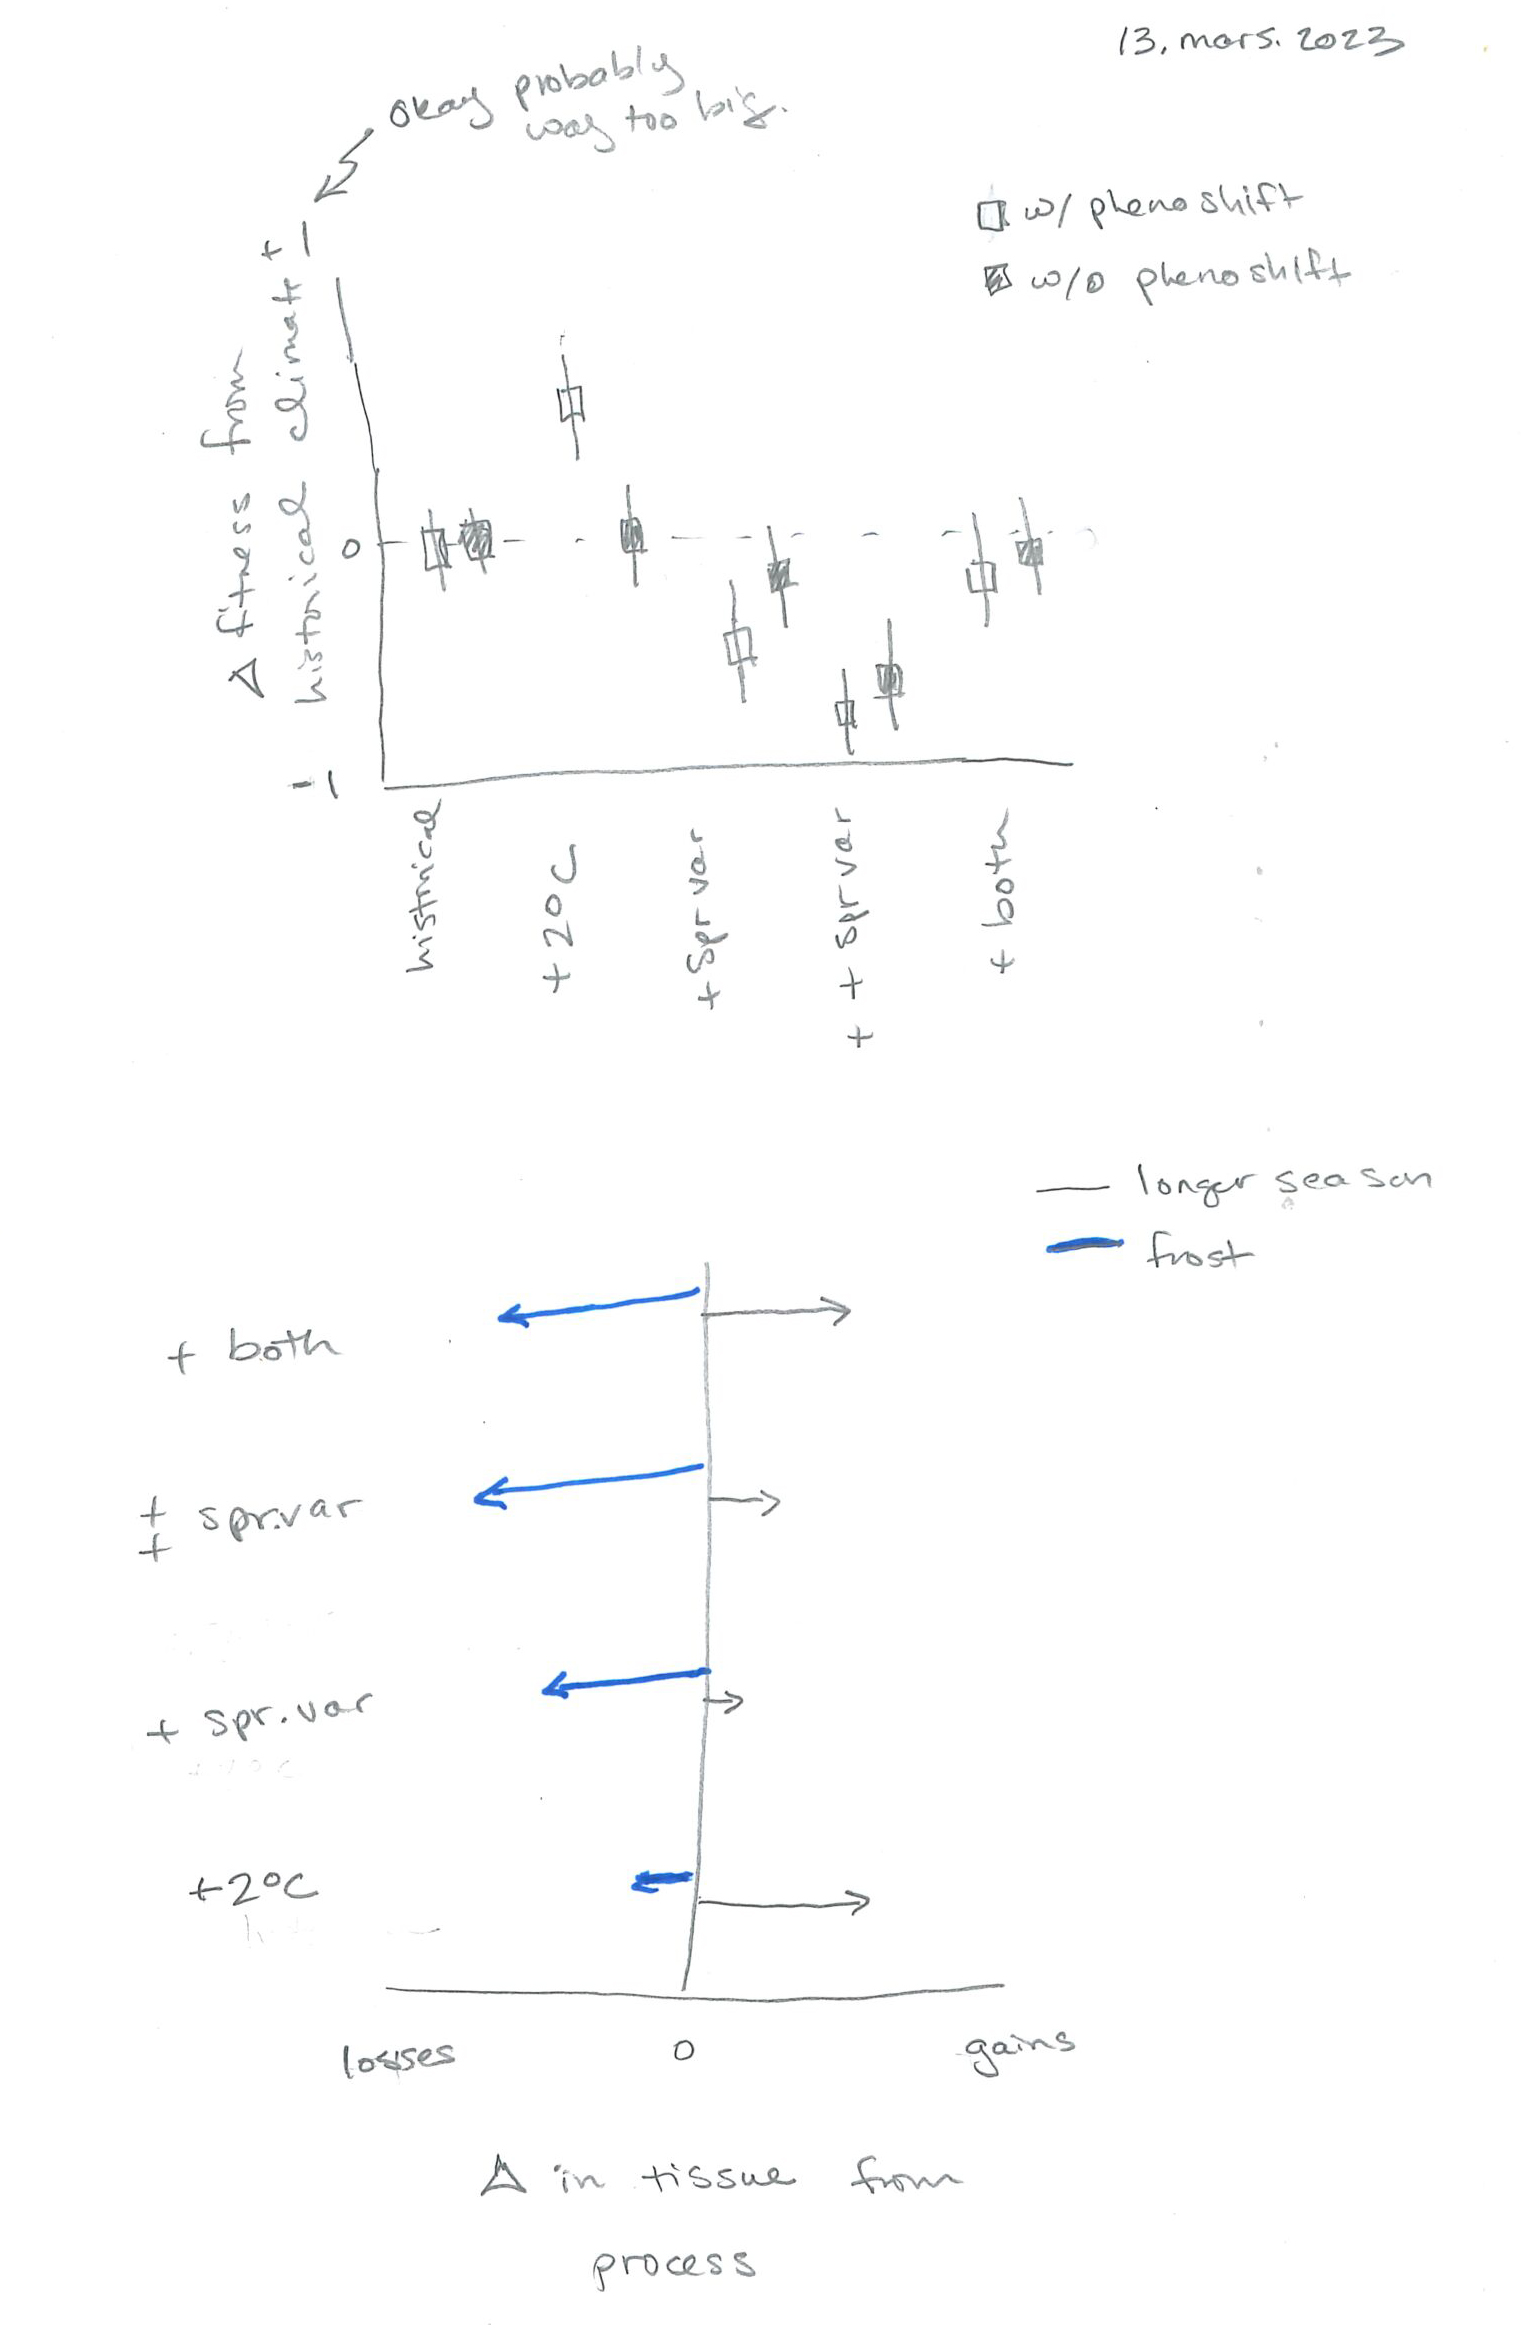
\includegraphics[width=0.75\textwidth]{figures/2023Mar13Notes.jpg}
  \end{center}
  \caption{My cheap figure showing graphs we'd like to make. Asses overall shifts in fitness due to mean warming versus increased variability (leading to discrete events), then break down how much of those shifts are due to changes in growing season length (which I assume are always positive, but I may be wrong) versus tissue lost to frost.}
\label{fig}
\end{figure}
\vspace{-1ex}

\end{document}

{\bf What is basically done}
\begin{enumerate}
\item Have a running model (and can get all the climate data we need for historical and future simulations): PhenoFit 4
\item Picked species
\end{enumerate}

\vspace{-1ex}
\begin{figure}
  \begin{center}
\includegraphics[width=1\textwidth]{figures/sabbfig.png}
  \end{center}
  \caption{Climate change alters the depth and timing of cold hardiness (the maximum temperature tissues can withstand before death, shown here as `lower lethal temperature') and critical growing season events, reshaping how hardiness and phenology interact with climate to determine growth, reproduction and survival. (A) a hypothetical pre-climate year includes several freeze events early in the year, but temperatures are never beyond the plant's maximum during major events; in contrast (B), a year with warming has fewer freeze events, earlier and accelerated budburst and flowering, but slower ripening and the potential loss of fruit due to heat extremes. }
\label{fig}
\end{figure}
\vspace{-1ex}